\newlength{\teaserheight}
\setlength{\teaserheight}{3.5cm}
\begin{strip}
    \vspace{-0.45cm}
    \centering
    \footnotesize%
    \begin{tabular}{ccc}
        \setlength{\tabcolsep}{0pt}
        \renewcommand{\arraystretch}{0.9}
        \hspace{-0.7cm}
        \begin{tabular}{c}
            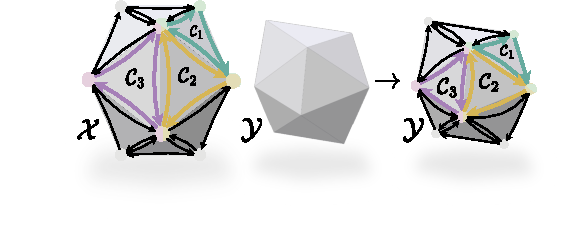
\includegraphics[width=6cm,trim={1.2cm 0.7cm 0 -1cm}]{figs/surface-cycles4.drawio.pdf}
        \end{tabular}
        &
        \hspace{-1cm}
        \adjustbox{trim=0 0 0 2cm}{%
            \begin{tabular}{ccc}
                 \includegraphics[height=\teaserheight]{figs/teaser/ours/DancingRunningMan272-DancingRunningMan285_M.png}
                 &
                 \hspace{-0.85cm}
                 \includegraphics[height=\teaserheight,trim={0 0 0 0.5cm}]{figs/teaser/cao/DancingRunningMan272-DancingRunningMan285_N.png}
                 &
                 \hspace{-0.95cm}
                 \includegraphics[height=\teaserheight,trim={0 0 0 0.5cm}]{figs/teaser/ours/DancingRunningMan272-DancingRunningMan285_N.png}
                 \\
                 Source& 
                 Cao~\etal 
                 &Ours 
            \end{tabular}
        }
        &
        \hspace{-1cm}
        \begin{tabular}{c}
            \adjustbox{trim=0 0.85cm 0 0.8cm}{%
                \newcommand{\runtimeLineWidth}{2pt}
\newcommand{\rtCplotWidth}{1.3\columnwidth}
\newcommand{\rtCplotHeight}{0.65\columnwidth}
\pgfplotsset{%
	label style = {font=\large},
	tick label style = {font=\large},
	title style =  {font=\Large},
	legend style={  fill= gray!10,
		fill opacity=0.6, 
		font=\large,
		draw=gray!20, %
		text opacity=1}
}
\begin{tikzpicture}[scale=0.5, transform shape]
	\begin{axis}[%
		width=\rtCplotWidth,
		height=\rtCplotHeight,
		scale only axis,
		grid=major,
	      legend style={
		 	%
		 	%
                at={(1.02,1.24)},
		 	anchor=north east,
		 	legend columns=3,
		 	legend cell align={left}},
		ylabel={{\large Runtime [s]  \textcolor{gray!40}{$\leftarrow$}}},
		xlabel={$\#$ of Faces of individual Triangle Meshes},
		xmin=50,
		xmax=1750,
		xtick={250, 500, 750, 1000, 1250, 1500, 1750},
		xtick scale label code/.code={},
		ymin=0,
		ymax=1000,
            ytick={0, 250, 500, 750, 1000},
		ylabel near ticks,
		]
		
		\addplot [color=windheusercolor, line width=\runtimeLineWidth]
		table[row sep=crcr]{%
50	5.3454752\\
100	78.5283646\\
150	683.8947292\\
200	2232.7588358\\
250	2964.2542276\\
		};
		\addlegendentry{\textcolor{black}{\windheuser}}

		\addplot [color=cPLOT0, tension=0.2, line width=\runtimeLineWidth]
		table[row sep=crcr]{%
0 0\\
50	1.66142253875732\\
100	4.6863883972168\\
150	21.2299663066864\\
200	37.7827697277069\\
250	58.980616235733\\
300	102.505135154724\\
350	222.499098205566\\
400	213.992396688461\\
450	288.231658172607\\
500	430.349188232422\\
550	511.202847003937\\
600	804.884549236298\\
650	810.355409288406\\
700	925.835303497314\\
750	1133.83003811836\\
800	1154.35633182526\\
		};
		\addlegendentry{\textcolor{black}{\smcomb}}
\node[color=discocolor,rotate=50] at (axis cs:950, 397) (b) {\textbf{]}};
\node[color=discocolor] at (axis cs:950, 450) (b) {\large OOM};
    \addplot [color=discocolor, line width=\runtimeLineWidth]
		table[row sep=crcr]{%
50	4.61538190841675\\
100	8.21245727539062\\
150	26.7098184585571\\
200	28.5115680217743\\
250	33.2058145523071\\
300	57.9440919399261\\
350	47.961816072464\\
400	63.5641473293304\\
450	64.881423664093\\
500	145.214042568207\\
550	117.714063596725\\
600	149.570569038391\\
650	158.672130632401\\
700	196.373429059982\\
750	235.609471654892\\
800	232.494430494308\\
850	521.386315727234\\
900	276.886437511444\\
950	397.95380282402\\
		};
		\addlegendentry{\textcolor{black}{\discomatch\ (GPU)}}

\addplot [color=cPLOT5,tension=0.2,line width=\runtimeLineWidth]
		table[row sep=crcr]{%
50	2.15893530845642\\
150	22.4732964038849\\
250	343.254711389542\\
350	87.7516279220581\\
450	323.576714754105\\
550	299.947786092758\\
650	564.656882047653\\
750	673.805225729942\\
800	855.316\\
850	1002.63\\
};
\addlegendentry{\textcolor{black}{\spidermatch\ (geo.)}}%
    \addplot [color=cPLOT5, dashed,line width=\runtimeLineWidth]
		table[row sep=crcr]{%
0 0\\
50	0.0727925300598145\\
150	0.80660080909729\\
250	2.79375910758972\\
350	6.1397168636322\\
450	11.0672917366028\\
550	20.6555211544037\\
650	33.8513643741608\\
750	43.3372287750244\\
850	53.6141972541809\\
950	77.4060039520264\\
1050	80.8316583633423\\
1150	131.65684223175\\
1250	142.600990772247\\
1350	195.615426063538\\
1450	201.480194091797\\
1550	226.529071331024\\
1650	373.353313565254\\
1750	379.037929415703\\
1850	412.055595397949\\
1950	578.553\\
		};
		\addlegendentry{\textcolor{black}{\spidermatch\ }}%
\addplot [color=ourcolor, smooth, tension=0.2, line width=\runtimeLineWidth]
  table[row sep=crcr]{%
50	0.382844209671021\\
150	3.03250408172607\\
250	9.37670803070068\\
350	12.2255246639252\\
450	21.535619020462\\
550	34.291276216507\\
650	48.6560304164886\\
750	66.5410633087158\\
850	88.2784218788147\\
950	111.767062902451\\
1050	139.437685012817\\
1150	169.960187673569\\
1250	204.876774072647\\
1350	253.960168838501\\
1450	303.68256020546\\
1550	351.137157678604\\
1650	423.827531814575\\
1750	498.286844372749\\
1850	586.620145082474\\
};
\addlegendentry{\ours}
\end{axis}
\end{tikzpicture}%

            }
        \end{tabular}
        \\
        Key Idea of Our Approach
        &
        \hspace{-0.5cm}
        Triangulation Transfer via Computed Matchings
        &
        Runtime Comparison on FAUST Dataset
    \end{tabular}
    \vspace{-0.1cm}
    \captionof{figure}{
        \textbf{Left:} Illustration of our approach for geometrically consistent matching of 3D shape $\meshX$ to 3D shape $\meshY$. We represent shape $\meshX$ using $n$ surface cycles $\contour_1,\dots,\contour_n$ and then consistently match these  to shape $\meshY$ while  preserving neighbourhood relations between the cycles.
        \textbf{Middle:} The triangulation transfer between shapes using computed matchings of Cao~\etal~\cite{cao2023unsupervised}  (not geometrically consistent) and ours (geometrically consistent) illustrates the importance of geometric consistency. %
        \textbf{Right:} Our method is the first 3D shape matching approach that yields globally geometrically consistent matchings, that is globally optimal, and scalable in practice, opposed to all competing methods (the dashed line indicates a weak notion of geometric consistency, see explanation of methods in \cref{sec:experiments}).
    }
    \label{fig:teaser}
\end{strip}